\documentclass[11pt]{exam}
\usepackage[utf8]{inputenc}
\usepackage[a4paper,top=2cm,left=2cm,right=2cm,bottom=2cm]{geometry}
\usepackage{import}
\usepackage[T1]{fontenc}
\usepackage[german,ngerman]{babel}
\usepackage[table]{xcolor}
\usepackage{amsthm, esvect}
\usepackage{mathtools}
\RequirePackage{amssymb, amsfonts, amsmath, latexsym, verbatim, xspace}
\usepackage{systeme}
\usepackage{multicol}
\usepackage{multirow}
\usepackage{framed}
\usepackage{array}
\usepackage{ragged2e}
\usepackage{graphicx}
\usepackage{pdflscape}
\usepackage{epstopdf}
\usepackage{booktabs}
\usepackage{pdfpages}
\usepackage{float} % Allows putting an [H] in \begin{figure} to specify the exact location of the figure
\usepackage{wrapfig} % Allows in-line images such as the example fish picture
\usepackage{tikz, graphicx} % tikz
\usepackage[position=top]{subfig}
\usepackage[bookmarks=true]{hyperref}%Links
\usepackage{enumerate}
\usepackage{enumitem}
\usepackage[german,ruled,vlined,linesnumbered,algosection]{algorithm2e}
\usepackage[labelfont=sf]{caption}
\usepackage{lmodern}
\usepackage{lscape}
\usepackage{tabularx}
\usepackage{systeme}
\usepackage{hhline}
\usepackage{subfiles}
\usepackage{stackengine}
\usepackage{setspace}
\usepackage{MnSymbol}
\usepackage{tcolorbox}
\usepackage{bbm}
\usepackage{url}
\usepackage{xparse}
\usepackage{sectsty}
\usepackage{array}
\usepackage{ragged2e}
\usepackage{listings} %Stellt Code-Snippets sauber dar

% definiert die Sprache
\selectlanguage{German}

% add command for different dates in Swiss fashion
\newcommand{\monthwordlong}[1]{\ifcase#1 \or Januar\or Februar\or März\or April\or Mai\or Juni\or Juli\or August\or September\or Oktober\or November\or Dezember\fi}
\newcommand{\monthwordshort}[1]{\ifcase#1\or Jan\or Feb\or Mar\or Apr\or Mai\or Jun\or Jul\or Aug\or Sept\or Okt\or Nov\or Dez\fi}
\newcommand{\datelong}{\number\day.\:\monthwordlong{\the\month}\:\number\year}
\newcommand{\dateshort}{\number\day.\:\monthwordshort{\the\month}\:\number\year}

% define color of links inside a text
\definecolor{linkblue}{RGB}{0, 0, 80}
\definecolor{plotblue}{RGB}{100, 100, 255}
\definecolor{myblue}{RGB}{8,164,214}
\definecolor{myred}{RGB}{143,42,41}
\definecolor{forestgreen}{RGB}{34,139,34}
\definecolor{highdive}{RGB}{10,169,194}
\definecolor{charcoal}{RGB}{74,74,74}
\hypersetup{
	colorlinks=true,
	linkcolor=linkblue,
	filecolor=magenta,
	urlcolor=plotblue,
	citecolor=linkblue,
	pdfpagemode=FullScreen,
}


\lstdefinestyle{mystyle}{ % definiert den style des Code-Snippets
	%backgroundcolor=\color{backcolour},
	%commentstyle=\color{codegreen},
	%keywordstyle=\color{magenta},
	%numberstyle=\tiny\color{codegray},
	%stringstyle=\color{codepurple},
	basicstyle=\ttfamily\footnotesize,
	breakatwhitespace=false,
	breaklines=true,
	captionpos=b,
	keepspaces=true,
	%numbers=left,
	%numbersep=5pt,
	showspaces=false,
	showstringspaces=false,
	showtabs=false,
	tabsize=4
}
\lstset{style=mystyle}
\qformat{\Large\textbf{Aufgabe \thequestion\hfill\thepoints}}
\newlist{partes}{enumerate}{3}
\setlist[partes]{label=(\alph*)}
\newcommand{\parte}{\item}
\newlist{subpartes}{enumerate}{3}
\setlist[subpartes]{label=\roman*)}
\newcommand{\subparte}{\item}
\setlist[enumerate,1]{%(
	leftmargin=*, itemsep=12pt, label={\textbf{\arabic*.)}}}
\newcommand\answerbox{%%
	\fbox{\rule{2in}{0pt}\rule[-0.1ex]{0pt}{4ex}}}
\pointpoints{Punkt}{Punkte}
\hqword{Frage:}
\hpword{Mögliche Punkte:}
\hsword{Erreicht:}
\htword{Total}
\renewcommand*\half{.5}
\renewcommand{\solutiontitle}{\noindent\textbf{Lösung:}\par\noindent}

% Graphed boxes
\newcommand{\karos}[2]{
  \begin{tikzpicture}
    \draw[step=0.4cm,color=cyan,dotted] (0,0) grid (#1 cm ,#2 cm);
  %  \draw((#1)/2 cm,0)--((#1)/2 cm,/#2)/2cm)
  \end{tikzpicture}
}
\usetikzlibrary{arrows, petri, topaths, graphs}
\linespread{1.2} % Line spacing

%=========================================================
\newenvironment{parcols}[1][]{
    \begin{parts}\begin{multicols}{#1}
}{
    \end{multicols}\end{parts}
}
%=========================================================
\newenvironment{itemcols}[1][]{
	\begin{itemize}\begin{multicols}{#1}
		}{
	\end{multicols}\end{itemize}
}

%=========================================================
\newcommand{\antwort}[1]{
	{\setlength{\textwidth}{\textwidth}\fillwithgrid{#1cm}\vspace{5pt}}
}

%=========================================================
% Karriertes Papier für Antwort MIT OVERLAY
\tcbuselibrary{breakable,skins}
\usetikzlibrary{mindmap,trees}
\newlength\tindent
\setlength{\tindent}{\parindent}
\setlength{\parindent}{0pt}
\setlength{\parskip}{0pt}

\newtcolorbox{gridspace}[1]{%
	enhanced,
	breakable,
	blanker,
	boxrule=0pt,
	left=5mm,
	right=5mm,
	top=5.75mm,
	bottom=0mm,
	boxsep=0pt,
	height=#1cm,
	width=16cm,
	before upper={
		\begingroup
		\setlength{\baselineskip}{5.75mm}
		\setlength{\parskip}{0pt}
		\setlength{\lineskip}{0pt}
		% keep every paragraph on the grid rhythm
		%\everypar{\vspace{0pt}\strut}
		% math formulas shifted by one grid row
		\let\oldbracketopen\[
		\renewcommand{\[}{\vspace{-5mm}\oldbracketopen}
		% Align displayed formulas to the grid
		\setlength{\abovedisplayskip}{0pt}
		\setlength{\belowdisplayskip}{0pt}
		\setlength{\abovedisplayshortskip}{0pt}
		\setlength{\belowdisplayshortskip}{0pt}
		% Enumerate follows the same rhythm
		\setlist[enumerate]{leftmargin=6mm,itemsep=0mm,topsep=0pt,parsep=0pt,partopsep=0pt}
		\setlist[itemize]{leftmargin=6mm,itemsep=10mm,topsep=0pt,parsep=0pt,partopsep=0pt}},
	after upper={
		\endgroup},
	underlay={
		\draw[step=5mm,color=gray!55] (interior.south west) grid (interior.north east);}
}

\pagestyle{headandfoot}
\firstpageheader{}{}{\teacher}
\runningheader{}{}{\teacher}
\firstpagefooter{}{}{Seite \thepage\:von \numpages}
\runningfooter{}{}{Seite \thepage\:von \numpages}
%%
% Math Arrows
%%
\newcommand{\same}{\ensuremath{\Longleftrightarrow}}
\renewcommand{\to}{\ensuremath{\longrightarrow}}
\newcommand{\qsame}{\quad\same\quad}
\newcommand{\dsame}{\ensuremath{:\Leftrightarrow}}
\newcommand{\qdsame}{\quad\dsame\quad}
\newcommand{\ldsame}{\ensuremath{:\Longleftrightarrow}}
\newcommand{\samedef}{\ensuremath{\us {\text{def}} \Leftrightarrow}}
\newcommand{\qsamedef}{\quad\samedef\quad}
\newcommand{\lsamedef}{\ensuremath{\us {\text{def}} \Longleftrightarrow}}
\newcommand{\qlsamedef}{\quad\lsamedef\quad}


%%
% Mengendefinitionen
%%
\newcommand{\M}{\ensuremath{\mathcal{M}}}
\newcommand{\N}{\ensuremath{\mathbb{N}}}
\newcommand{\Z}{\ensuremath{\mathbb{Z}}}
\newcommand{\Q}{\ensuremath{\mathbb{Q}}}
\newcommand{\I}{\ensuremath{\mathbb{I}}}
\newcommand{\R}{\ensuremath{\mathbb{R}}}
\newcommand{\C}{\ensuremath{\mathbb{C}}}
\renewcommand{\S}{\ensuremath{\mathbb{S}}}
\newcommand{\Prim}{\ensuremath{\mathbb{P}}}
\newcommand{\0}{\ensuremath{\emptyset}}
\renewcommand{\Re}{\ensuremath{\operatorname{Re}}}
\renewcommand{\Im}{\ensuremath{\operatorname{Im}}}
\newcommand{\strich}{\ensuremath{\big\vert}}

%%
% Mengenoperation
%%
\renewcommand{\nin}{\not\in}


%%
% Logisches Und und Oder
%%
\newcommand{\sand}{\ensuremath{\; \land \;}}
\newcommand{\sor}{\ensuremath{\; \lor \;}}
\renewcommand{\*}{\ensuremath{\cdot}}
\newcommand{\oder}{\vee}
\newcommand{\n}{\neg}
\newcommand{\und}{\wedge}


%%
% Bei Integral, Summe,... die Grenzen über bzw.
% unter das Zeichen
%%
\renewcommand{\d}[1]{\ensuremath{\operatorname{d}\!{#1}}}
\newcommand{\Sum}{\sum\limits}
\newcommand{\Prod}{\prod\limits}
\newcommand{\Min}{\min\limits}
\newcommand{\Max}{\max\limits}
\newcommand{\Lim}{\lim\limits}
\newcommand{\Inf}{\inf\limits}
\newcommand{\Sup}{\sup\limits}
\newcommand{\Liminf}{\liminf\limits}
\newcommand{\Limsup}{\limsup\limits}
%\renewcommand{\Cup}{\bigcup\limits}
%\renewcommand{\Cap}{\bigcap\limits}
\newcommand{\Otimes}{\bigotimes\limits}
\newcommand{\Oplus}{\bigoplus\limits}


%%
% Arcus Cotangens, Logarithmus
%%
\let\oldsin\sin
\renewcommand{\sin}[1]{\oldsin{\left(#1\right)}}
\let\oldcos\cos
\renewcommand{\cos}[1]{\oldcos{\left(#1\right)}}
\let\oldtan\tan
\renewcommand{\tan}[1]{\oldtan{\left(#1\right)}}
\let\oldarcsin\arcsin
\renewcommand{\arcsin}[1]{\oldarcsin{\left(#1\right)}}
\let\oldarccos\arccos
\renewcommand{\arccos}[1]{\oldarccos{\left(#1\right)}}
\let\oldarctan\arctan
\renewcommand{\arctan}[1]{\oldarctan{\left(#1\right)}}
\let\oldln\ln
\renewcommand{\ln}[1]{\oldln{\left(#1\right)}}
\newcommand{\Log}[2]{\ensuremath{\operatorname{log}_{#1}\left(#2\right)}}
\newcommand{\e}{\operatorname{e}}
\renewcommand{\exp}[1]{\ensuremath{\operatorname{\e}^{#1}}}


%%
% Griechische Buchstaben
%%
\renewcommand{\epsilon}{\ensuremath{\varepsilon}}
\renewcommand{\phi}{\varphi}
\renewcommand{\l}{\lambda}
\renewcommand{\t}{\tau}


%%
% Bezeichnungen
%%
\newcommand{\Rgn}{\R_{>0}} % R grösser Null
\newcommand{\Rad}{\operatorname{Rad}}   % Radikal
\newcommand{\kgV}{\operatorname{kgV}}   % Kleinster gemeinsame Vielfache
\newcommand{\ggT}{\operatorname{ggT}}   % Grösster gemeinsame Teiler
\newcommand{\winkel}{\sphericalangle}          % Winkelsymbol
\DeclarePairedDelimiter\abs{\lvert}{\rvert} % besserer Betrag
\makeatletter
\let\oldabs\abs
\def\abs{\@ifstar{\oldabs}{\oldabs*}}
\makeatother


%%
% Vektorgeometrie
%%
\renewcommand{\v}[1]{\vv{#1}}       % besserer Pfeil über Buchstaben
\renewcommand{\vec}[2]{\begingroup\renewcommand{\arraystretch}{1}\left(\begin{array}{c} #1 \\ #2 \end{array}\right)\endgroup}   % two dimensional vector
\renewcommand{\Vec}[3]{\begingroup\renewcommand{\arraystretch}{1}\left(\begin{array}{c} #1 \\ #2 \\ #3 \end{array}\right)\endgroup}      % three dimensional vector


%%
% Text
%%
\newcommand*{\Ueq}[1]{\mathrel{\mathop{=}\limits_{\text{#1}}}}
\newcommand*{\Oeq}[1]{\mathrel{\stackrel{\text{#1}}{=}}}
\newcommand{\utext}[2]{\underbrace{#1}_{\substack{#2}}}
\newcommand{\otext}[2]{$\overbrace{\textrm{#1}}^{\textrm{#2}}$}
\newcommand{\lineortext}[1]{\hspace{0,1cm}\underline{\hspace{0.1cm}\hphantom{#1}\hspace{0.1cm}}\hspace{0,1cm}} % Lückentext erstellen
\newcommand{\gap}[1]{\rule{#1 cm}{1pt}}
%=========================================================
\newcommand{\theme}{Wachstum \& Zerfall}
\newcommand{\teacher}{Jonas Guler}
\graphicspath{{data-algebra/}} % Setzt den Pfad zu den Bilder fest
%=========================================================
\begin{document}
\fontsize{14}{14}\selectfont
\begin{center}
    \huge\bf\theme
\end{center}

\begin{questions}
%=========================================================
%-------------------TESTFRAGEN
%=========================================================
\question[3]
Entschiede, ob die folgenden Funktionen eine Exponentialfunktion sind. Begründe deine Antwort.
\begin{parcols}[3]
    \part $y=3^{x-1}$
    \part $y=-3x+1$
    \part $y=\sqrt{3}^x+\frac{2}{3}$
    \part $y=0.2^{-x}$
    \part $y=2\*\left(\frac{1}{2^x}\right)$
    \part $y=x^3$
\end{parcols}

%---------------------------------------------------------
\question[3]
Entschiede, ob die folgenden Funktionen eine Exponentialfunktion sind. Begründe deine Antwort.
\begin{parcols}[3]
    \part $y=3^{x-1}$
    \part $y=x^3$
    \part $y=0.2^{-x}$
    \part $y=2\*\left(\frac{1}{2}\right)^x-2$
    \part $y=-3x+1$
    \part $y=\sqrt{3}^x+\frac{2}{3}$
\end{parcols}

%---------------------------------------------------------
\question[2]
Beschreibe in eigenen Worten, unter welcher Bedingung eine Funktion der Form $f(x)=b\*a^x$ wachsend bzw. fallend ist. Veranschauliche deine Aussage anhand zwei geeigneter Beispiele.

%---------------------------------------------------------
\question[2]
Skizziere die beiden Funktionen $f(x)=1.3^x$ und $g(x)=\left(\frac{1}{3}\right)^x$
\begin{figure}[H]
    \hspace{1cm}
    \begin{tikzpicture}[cross/.style={draw, cross out, minimum size=2*(#1-1pt), inner sep=0pt, outer sep=0pt}, x=10mm, y=5mm,
        >=latex,   %Voreinstellung für Pfeilspitzen
        font=\footnotesize, scale=1]
        %Raster zeichnen
        \draw [color=gray!50]  [step=5mm] (-4.3,-1.3) grid (4.3,16.3);
        % Achsen zeichnen
        \draw[->,thick] (-4.3,0) -- (4.8,0) node[left, below] {\normalsize $x$};
        \draw[->,thick] (0,-1.3) -- (0,17.3) node[above, left=4pt] {\normalsize $y$};
        % Achsen beschriften
        \foreach \x in {-4,-3,-2,-1,1,2,3,4} \draw (\x,-.2) -- (\x,.2) node[below=4pt] {$\x$};
        \foreach \y in {2,4,...,16} \draw (-.1,\y) -- (.1,\y) node[left=4pt] {$\y$};
        % Besserer Ursprung
        \draw[color=black] (0pt,-7pt) node[left] {$0$};
        %Funktionen zeichnen:
        \clip(-4.3,-1.3) rectangle (4.3,10.3); %Bildbereich
        %Beschriftung
        %\node[forestgreen]  at (3.2,1) {\normalsize$g$};
    \end{tikzpicture}
\end{figure}

%---------------------------------------------------------
\question[2]
Skizziere die beiden Funktionen $f(x)=1.5^x$ und $g(x)=\left(\frac{2}{3}\right)^x$
\begin{figure}[H]
    \hspace{1cm}
    \begin{tikzpicture}[cross/.style={draw, cross out, minimum size=2*(#1-1pt), inner sep=0pt, outer sep=0pt}, x=10mm, y=5mm,
        >=latex,   %Voreinstellung für Pfeilspitzen
        font=\footnotesize, scale=1]
        %Raster zeichnen
        \draw [color=gray!50]  [step=5mm] (-4.3,-1.3) grid (4.3,16.3);
        % Achsen zeichnen
        \draw[->,thick] (-4.3,0) -- (4.8,0) node[left, below] {\normalsize $x$};
        \draw[->,thick] (0,-1.3) -- (0,17.3) node[above, left=4pt] {\normalsize $y$};
        % Achsen beschriften
        \foreach \x in {-4,-3,-2,-1,1,2,3,4} \draw (\x,-.2) -- (\x,.2) node[below=4pt] {$\x$};
        \foreach \y in {2,4,...,16} \draw (-.1,\y) -- (.1,\y) node[left=4pt] {$\y$};
        % Besserer Ursprung
        \draw[color=black] (0pt,-7pt) node[left] {$0$};
        %Funktionen zeichnen:
        \clip(-4.3,-1.3) rectangle (4.3,10.3); %Bildbereich
        %Beschriftung
        %\node[forestgreen]  at (3.2,1) {\normalsize$g$};
    \end{tikzpicture}
\end{figure}

%---------------------------------------------------------
\question[3]
Im folgenden sind drei Wertetabellen gegeben. Entscheide für jede Wertetabelle, ob es sich um eine Exponentialfunktion handelt. Wenn ja, gib die Funktionsgleichung an.
\begin{parcols}[3]
    \part \
        \begin{table}[H]
            \begin{tabular}{|c|c|c|c|c|}\hline
                $x$ & 1 & 2 & 3 & 4 \\\hline
                $f(x)$ & 4 & 16 & 64 & 256 \\\hline
            \end{tabular}
        \end{table}
    \part \
        \begin{table}[H]
            \begin{tabular}{|c|c|c|c|c|}\hline
                $x$ & 1 & 2 & 3 & 4 \\\hline
                $f(x)$ & -6 & 2 & 10 & 18 \\\hline
            \end{tabular}
        \end{table}
    \part\
        \begin{table}[H]
            \begin{tabular}{|c|c|c|c|c|}\hline
                $x$ & 1 & 2 & 3 & 4 \\\hline
                $f(x)$ & 20 & 5 & $\frac{5}{4}$ & $\frac{5}{16}$ \\\hline
            \end{tabular}
        \end{table}
\end{parcols}

%---------------------------------------------------------
\noaddpoints
\question[\totalpoints]
\addpoints
Beantworte für die beiden Funktionen $f:y=a\*x$ und $g:y=a^x$ die folgenden Fragen: Wie verändert sich der Funktionswert, ...
\begin{parts}
    \part[2] ... wenn man den $x-$Wert um 6 erhöht?
    \part[2] ... wenn man den $x-$Wert um 4 verkleinert?
\end{parts}


%---------------------------------------------------------
\noaddpoints
\question[\totalpoints]
\addpoints
Beantworte für die beiden Funktionen $f:y=a\*x$ und $g:y=a^x$ die folgenden Fragen: Wie verändert sich der Funktionswert, ...
\begin{parts}
    \part[2] ... wenn man den $x-$Wert um 4 erhöht?
    \part[2] ... wenn man den $x-$Wert halbiert?
\end{parts}

%---------------------------------------------------------
\noaddpoints
\question[\totalpoints]
\addpoints
Betrachte die beiden Funktionen $f:y=a\*x$ und $g:y=a^x$. Wie lautet die Funktionsgleichung, wenn bei jeder Erhöhung von $x$ um $1$ ...
\begin{parts}
    \part[2] ... der Funktionswert verdreifacht wird?
    \part[2] ... der Funktionswert um $20\%$ zunimmt?
\end{parts}


%---------------------------------------------------------
\question[6]
Ordne die Graphen den Funktionsgleichungen zu. Begründe deine Antwort.\\
\begin{minipage}{0.45\linewidth}
    \centering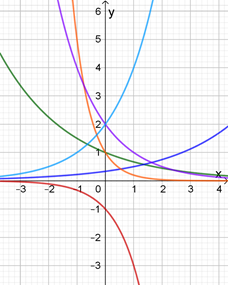
\includegraphics[scale=3]{expGraph.png}
\end{minipage}
\hfill
\begin{minipage}{0.45\linewidth}
    \begin{parts}
    \part $f_1(x)=2\cdot0.5^x$
    \part $f_2(x)=-3^x$
    \part $f_3(x)=\left(\frac{2}{3}\right)^x$
    \part $f_4(x)=\frac{1}{3}\cdot1.5^x$
    \part $f_5(x)=0.2^x$
    \part $f_6(x)=2\cdot 2^x$
\end{parts}
\end{minipage}

%---------------------------------------------------------
\question[4]
Am Eröffnungstag eines Streichelzoos befanden sich $93$ Meerschweinchen in einem Gehege. Ein Jahr später waren es bereits $115$.
\begin{parts}
    \part Wie viele Meerschweinchen werden es am Tag des $10-$jährigen Jubiläums sein, wenn wir ein lineares Wachstum annehmen?
    \part Wie viele Meerschweinchen werden es an diesem Tag sein, wenn wir ein exponentielles Wachstum annehmen?
\end{parts}


%---------------------------------------------------------
\question[4]
In einem See verringert sich die Intensität des Lichtes mit jedem Meter Wassertiefe um $40\%$.
\begin{parts}
    \part Stelle ein Zerfallsgesetz auf, das die Wassertiefe in Meter der Lichtintensität in Prozent zuordnet.
    \part In welcher Wassertiefe beträgt die Lichtintensität noch $5\%$ der Intensität über der Wasseroberfläche?
\end{parts}

%---------------------------------------------------------
\question[4] %DMK 9-10 A25
Ein Kapital von $1000.-$ CHF wird bei einer Bank angelegt. Der Zins wird jeweils am Ende der Zinsperiode zu Kapital addiert. Berechne das Kapital nach 10 Jahren, wenn...
\begin{parts}
    \part ... das Kapital jährlich zu $1\%$ verzinst wird.
    \part ... das Kapital monatlich zu $\frac{1}{12}\%$ verzinst wird.
\end{parts}
Welche Variante würdest du bevorzugen? Begründe.

%---------------------------------------------------------
\question[5]
Von einem neu entdeckten radioaktiven Element namens Heerbruggium zerfallen in $7$ Minuten $10\%$ seines noch vorhandenen Bestandes.
\begin{parts}
    \part Berechne seine Halbwertszeit.
    \part Wie viel Prozent seines noch vorhandenen Bestandes zerfallen in der nächsten Stunde?
\end{parts}

%---------------------------------------------------------
\question[6]
Die Vermehrung von Keimen in Kuhmilch lässt sich durch eine Exponentialfunktion beschreiben. In $1$ cm$^3$ Kuhmilch werden $3$ Stunden nach dem Melken $66'000$ Keime nachgewiesen. $2$ Stunden später sind es bereits $1.1$ Millionen Keime.
\begin{parts}
    \part Berechne die Anzahl der Keime $6$ Stunden nach dem Melken.
    \part In welcher Zeit verdreifacht sich die Anzahl der Keime?
    \part Um wie viele Prozent wächst die Anzahl der Keime innerhalb einer Stunde?
\end{parts}

%---------------------------------------------------------
\question[4] %Ss
Eine Pilzkultur an einer Kellerwand wird in einem Beobachtungszeitraum von drei Monaten chemisch so behandelt, dass ihre Fläche jede Woche um $11\%$ abnimmt. Zu Beginn des Zeitraums bedeckt sie eine Fläche von $2.4\:m^2$.
\begin{parts}
    \part Welche Fläche bedeckt sie am Ende des Beobachtungszeitraums?
    \part Wie viele Tage muss die Behandlung insgesamt dauern, dass die Pilzkultur höchstens noch eine Fläche von $0.1\:m^2$ bedeckt?
\end{parts}

%---------------------------------------------------------
\question[6]
Die Entwicklung der wöchentlichen Corona-Fallzahlen verlief in gewissen Zeiträumen annähernd exponentiell. Im Jahr $2021$ wurden in der Kalenderwoche $44$ insgesamt $17'203$ und in der Kalenderwoche $45$ insgesamt $24'823$ positive Fälle gemeldet. Unter der Annahme eines exponentiellen Wachstums der positiven Fälle berechne das Folgende:
\begin{parts}
    \part Bestimme die prozentuale wöchentliche Zunahme.
    \part Wie viele Fälle sind in der Kalenderwoche $48$ zu erwarten?
    \part In welchem Zeitraum (in Tagen) verdoppeln sich die positiven Fälle?
    \part Wir nehmen an, das exponentielle Wachstum setzt sich ungebremst fort. In welcher Kalenderwoche wäre erstmals mit mehr als $250'000$ Fälle pro Woche zu rechnen?
\end{parts}

%---------------------------------------------------------
\question[4] %Ss
Faltet man ein Stück Papier im DIN Format mehrfach längs der Mittellinie, so liegen erst zwei, dann vier Schichten,... übereinander. Es wird dabei immer kleiner und dicker. Wie oft müsste das Blatt gefaltet werden, um einen Turm, der bis zum Mond reicht, zu erhalten?\\
(Entfernung zum Mond: $384'000\:km$, Papierdicke: $0.1\:mm$)

%---------------------------------------------------------
\question[4] %DMK 9-10 A25
Ein Kapital von $1000.-$ CHF wird bei einer Bank angelegt. Der Zins wird jeweils am Ende der Zinsperiode zu Kapital addiert. Berechne das Kapital nach 10 Jahren, wenn
\begin{itemize}
    \item das Kapital jährlich zu $1\%$ verzinst wird.
    \item das Kapital monatlich zu $\frac{1}{12}\%$ verzinst wird.
\end{itemize}
Vergleiche nun die beiden Zinsvarianten. Welche Variante würdest du bevorzugen? Begründe.

%---------------------------------------------------------
\question[6]
Vor $10$ Jahren betrug der Holzbestand eines Waldes $7'000$ m$^3$. Ohne Abholzen ist er inzwischen auf $9'880$ m$^3$ angewachsen. Man darf annehmen, dass daas Holzwachstum ein exponentieller Vorgang ist.
\begin{parts}
    \part Bestimme die jährliche Wachstumsrate.
    \part Berechne die Zeitspanne, innerhalb der sich der Holzbestand verdoppelt.
    \part Der Besitzer plant, in $3$ Jahren $3'000$ m$^3$ Holz zu schlagen. Wann wird dieser Wald den heutigen Holzbestand wieder erreichen.
\end{parts}

%---------------------------------------------------------
\noaddpoints
\question[\totalpoints] %NeueWege
\addpoints
Im Jahr $1950$ lebten $2.5$ Milliarden Menschen auf der Erde, $1980$ waren es dann $4.5$ Milliarden.
\begin{parts}
    \part[2] Stelle eine Wachstumsfunktion auf, die das Bevölkerungswachstum oben beschreibt.
    \part[2] Bestimme die Verdoppelungszeit
    \part[2] Vergleiche dein Resultat mit den Daten von $2005$ ($6.4$ Milliarden) und $1920$ ($1.8$ Milliarden). Was fällt dir auf?
    \part[2] $2005$ prognostizierten Experten der Vereinten Nationen bis zum Jahr $2050$
    einen Anstieg auf $9.1$ Milliarden. Wie lautet deine Prognose?
\end{parts}

%---------------------------------------------------------
\question[6]
Im Jahr $1945$ lebten $4.2$ Millionen Menschen in der Schweiz, $1967$ waren es dann $6.9$ Millionen.
\begin{parts}
    \part Stelle eine Wachstumsfunktion auf, die den Prozess oben beschreibt.
    \part Bestimme die Verdoppelungszeit.
    \part Vergleiche das Wachstum aus (a) mit den neuen erhobenen Daten von $2005$ ($7.3$ Millionen) und $1900$ ($3.4$ Millionen). Beschreibe in eigenen Worten, was dir dabei auffällt.
\end{parts}

%---------------------------------------------------------
\question[8]
\begin{parts}
    \part Im Jahr $1945$ lebten $4.2$ Millionen Menschen in der Schweiz, $1967$ waren es dann $6.9$ Millionen. Modelliere das Bevölkerungswachstum und bestimme die Verdoppelungszeit.
    \part Vergleiche das Wachstum aus (a) mit den neuen Daten von $2005$ ($7.3$ Millionen) und $1900$ ($3.4$ Millionen). Was fällt dir auf?
    \part $2005$ prognostizierten Experten des Bundesamtes für Statistik bis zum Jahr $2050$ einen Anstieg auf $9.5$ Millionen. Wie lautet deine Prognose?
\end{parts}

%---------------------------------------------------------
\noaddpoints
\question[\totalpoints]
\addpoints
Eine Computeranlage mit Neuwert $2056900.-$ CHF wird nach $6.5$ Jahren für $400000.-$ CHF verkauft.
\begin{parts}
    \part[2] Wie viel Prozent beträgt die mittlere jährliche Wertabnahme?
    \part[3] Nach $20$ Jahren möchten neue Investoren die Anlage wieder auf den neusten Stand bringen. Wie viel Geld müssten investiert werden, um wieder auf den Neuwert zu gelangen?
\end{parts}

%---------------------------------------------------------
\question[2]
Entscheide in der Tabelle unten, ob die Aussagen wahr oder falsch sind. Die Antworten müssen nicht begründet werden.\newline
\begin{small}
    Bewertung: Für $0-2$ korrekte Antworten gibt es keine Punkte; $3$ korrekte Antworten einen Punkt und falls alle Antworten korrekt sind, gibt es $2$ Punkte.
\end{small}
\begingroup
\renewcommand{\arraystretch}{1.5}
\begin{table}[h]
    \centering
    \begin{tabular}{|p{12cm}|c|c|}\hline
         & wahr & falsch \\\hline
        Wenn eine Grösse jährlich um $7\%$ wächst, dann wächst sie in zwei Jahren um exakt 14\%. & & \\\hline
        Eine Funktion $f(t)=200\*0.65^t$ beschreibt einen exponentiellen Prozess, bei dem eine Grösse pro Zeiteinheit um $35\%$ abnimmt. & & \\\hline
        Eine Funktion $f(t)=200\*1.7^t$ beschreibt einen exponentiellen Prozess, bei dem eine Grösse pro Zeiteinheit um $170\%$ zunimmt. & & \\\hline
        Eine Funktion $f(t)=200\*\left(\frac{1}{\sqrt{2}}\right)^t$ beschreibt einen exponentiellen Prozess, bei dem sich eine Grösse alle zwei Jahre halbiert. & & \\\hline
        Eine Funktion $f(t)=200\*0.75^t$ beschreibt einen exponentiellen Prozess, bei dem eine Grösse pro Zeiteinheit um $25\%$ abnimmt. & & \\\hline
        Eine Funktion $f(t)=200\*\left(\frac{1}{\sqrt{2}}\right)^t$ beschreibt einen exponentiellen Prozess, bei dem sich eine Grösse alle zwei Jahre halbiert. & & \\\hline
        Wenn eine Grösse jährlich um $9\%$ wächst, dann wächst sie in zwei Jahren um exakt $18\%$. & & \\\hline
        Eine Funktion $f(t)=200\*1.7^t$ beschreibt einen exponentiellen Prozess, bei dem eine Grösse pro Zeiteinheit um $170\%$ zunimmt. & & \\\hline
        Wenn eine Grösse jährlich um $7\%$ wächst, dann wächst sie in zwei Jahren um exakt 14\%. & & \\\hline
        Eine Funktion $f(t)=200\*0.65^t$ beschreibt einen exponentiellen Prozess, bei dem eine Grösse pro Zeiteinheit um $35\%$ abnimmt. & & \\\hline
        Eine Funktion $f(t)=200\*1.7^t$ beschreibt einen exponentiellen Prozess, bei dem eine Grösse pro Zeiteinheit um $170\%$ zunimmt. & & \\\hline
        Eine Funktion $f(t)=200\*\left(\frac{1}{\sqrt{2}}\right)^t$ beschreibt einen exponentiellen Prozess, bei dem sich eine Grösse alle zwei Jahre halbiert. & & \\\hline
        Eine Funktion $f(t)=200\*0.55^t$ beschreibt einen exponentiellen Prozess, bei dem eine Grösse pro Zeiteinheit um $55\%$ abnimmt. & & \\\hline
        Eine Funktion $f(t)=200\*\left(\frac{1}{\sqrt{2}}\right)^t$ beschreibt einen exponentiellen Prozess, bei dem sich eine Grösse alle zwei Jahre halbiert. & & \\\hline
        Wenn eine Grösse jährlich um $10\%$ abnimmt, dann nimmt sie in zwei Jahren um exakt $19\%$ ab. & & \\\hline
        Eine Funktion $f(t)=200\*1.3^t$ beschreibt einen exponentiellen Prozess, bei dem eine Grösse pro Zeiteinheit um $30\%$ zunimmt. & & \\\hline
    \end{tabular}
\end{table}
\endgroup






\end{questions}
\end{document}